\subsection{Open Exhaustions in \texorpdfstring{$\Reals^n$}{n Dimensions}}
\label{sec::gen-OEX}
In this section we generalize the notion of an effective open exhaustion to that of $\Reals^n$ by generalizing intervals in $\Reals$ to cubes in $\Reals^n$.
\begin{definition}[Open $n$-cube]
    Let $I_1, \ldots, I_n \subseteq \Reals$ be open intervals. Then we call the open set $I_1\times \cdots \times I_n \subseteq \Reals^n$ an \emph{\openncube{}}.
\end{definition}
\begin{definition}[Closed $n$-cube]
    Let $I_1, \ldots, I_n \subseteq \Reals$ be closed intervals. Then we call the closed set $I_1\times \cdots \times I_n \subseteq \Reals^n$ a \emph{\closedncube{}}.
\end{definition}
\begin{definition}[Rational $n$-cube]
    Let $I_1, \ldots, I_n \subseteq \Reals$ be open (resp.\null{} closed) intervals. We call the open (resp.\null{} closed) set $I_1\times \cdots \times I_n \subseteq \Reals^n$ a \emph{\rationalopenncube{}} (resp.\null{} \rationalclosedncube{}) if all the endpoints of $I_1, \ldots, I_n$ are rational.
    The set $\mathbb{I}^n$ \index{$\mathbb{I}^n$} denotes the set of all rational $n$-cubes.
\end{definition}
\begin{definition}[\RealizabilityrelationonmathbbIton{}]
    We define the realizability relation ${
    \Vdash_{\mathbb{I}^n}}$ as the smallest relation satisfying
    \[
    \infer{
        c_1\Vdash_{\Rationals} a_1 \and c_2\Vdash_{\Rationals} b_1  \and \cdots \and c_{2n-1}\Vdash_{\Rationals} a_n \and c_{2n}\Vdash_{\Rationals} b_n
    }
    {
        p_1^{a_1}p_2^{b_1}\cdots p_{2n-1}^{a_n}p_{2n}^{b_n} \Vdash_{\mathbb{I}^n} (a_1,b_1)\times \cdots \times (a_n, b_n)
    }
    \]
    where $p_i$ is the $i$th prime number.
\end{definition}
Defining a realizability relation for $\mathbb{I}^n$ along with Definitions \ref{def::realizability-on-sequences},\ref{def::realizability-on-nats}  and Definition \ref{def::computability-on-assemblies} lets us define computable functions from $\Nats$ to finite sequences of cubes.

\begin{definition}[\Generalizedopenexhaustion{}] %with eventual covering
\label{def::generalized_open_exhaustion_with_eventual_covering}
    Let $U$ be an open subset of $\Reals^n$, and $X=(U_0, U_1, U_2,...)$ a sequence of open subsets of $\Reals^n$. The sequence $X$ is called an \textit{open exhaustion of $U$} iff
    \begin{enumerate}
        \item $ U = \bigcup_{i=0}^\infty U_i$, and
        \item for each $l \in \Nats$,
          $U_l$ is a (not necessarily disjoint) finite union of non-empty open $n$-cubes $Q_1^l, Q_2^l,...,Q_{k_l}^l $ 
          \item for any $l\in \Nats$ there is some $j>l\in \Nats$ such that $\overline{U_l} = \bigcup_{i=0}^{k_l} \overline{Q_i^l} \subseteq U_{j}$, and also $U_l \subseteq U_{l+1}$.
    \end{enumerate}
     For each $l\in\Nats$, $U_l$ is called a \emph{stage} of the exhaustion, with components $Q_1^l, Q_2^l,...,Q_{k_l}^l$. 
\end{definition}

\begin{definition}[Generalized effective open exhaustion]
\label{def::generalized-effecive-open-exhaustion}
An open exhaustion $(U_1, U_2, \ldots)$ of an open set $U\subseteq \Reals^n$ is called \textit{effective} if 
\begin{itemize}
    \item 
    each stage $U_l$ consists of finitely many open rational $n$-cubes $Q_1^l, \ldots, Q_{k_l}^l$, and
    \item the map
    \[
    l\mapsto (Q_1^l, \ldots, Q_{k_l}^l) 
    \]
    which delivers the sequence of stages 
    \[U_l = (Q_1^l, \ldots, Q_{k_l}^l)
    \]
    is recursive.
\end{itemize}
\end{definition}
\begin{remark}
    Note that the generalized notion of an effective open exhaustion in $\Reals^n$ given in Definition \ref{def::generalized-effecive-open-exhaustion} for the case where $n=1$,
    coincides with the concept of a 
    % \edchange{WK}{open exhaustion in $\Reals$ given earlier in Definition \ref{def::open_exhaustion}.}
    simple effective open exhaustion in $\Reals$ given earlier in Definition \ref{def::simple-effecive-open-exhaustion}
    % \edcomm{WK}{except that the recursive map is missing}.}
\end{remark}

\begin{definition}[\Effectivesequenceofopenexhaustions{}]
    Let $(U_0, U_1, \ldots)$ be a sequence of open sets in $\Reals^n$ each with an effective open exhaustion. We call the sequence $U_0, U_1, \ldots$ an \emph{effective sequence of open exhaustions} if we have a recursive function 
    \[
        \Stage : \Nats\times \Nats \to {(\mathbb{I}^n)}^*
    \]
    taking in the index $i$ of the open set, the stage $s$, and outputting the $n$-cubes in stage $s$ of the effective open exhaustion of $O_i$.
\end{definition}

\begin{theorem}[Union of effective open exhaustions]
    Let $(U_0, U_1, \ldots)$ be an effective sequence of open exhaustions. Then $\bigcup_{i\in\Nats}U_i$ has an effective open exhaustion.
\end{theorem}
\begin{proof}
    Let us assume the effective the open exhaustion for $U_0, U_1, \ldots$ is given by $(O_0), (O_1), \ldots$ and let us denote the $l$th stage of $(O_i)$ by $O_i^l$ (for $i \in \Nats$).\\

    Stage $t$ of the effective open exhaustion for $\bigcup_{i\in\Nats}U_i$ consists of the union of the first $t$ stages of the first $t$ open exhaustions.
    Let us construct the effective open exhaustion $(S_t)$ formally by 
    \[
    S_t = \bigcup_{k=0}^{t-1} O_k^t.
    \]
    We can clearly compute the above open exhaustion for $\bigcup_{i\in\Nats}U_i$ since each $O_k^t$ is a finite union of finitely many intervals.
\end{proof}

\begin{corollary}
\label{corollary::effectively_open_on_cubes_implies_effectively_open_on_open_sets}
    Let $f:\Reals^n \to \Reals^m$. Let us assume for any rational open $m$-cube $Q$ that $f^{-1}(Q)$ has an effective open exhaustion $(O_l^Q)$. If the function
    \[
    \mathit{Func}:\mathbb{I}^m\times\Nats\to{(\mathbb{I}^n)}^*
    \]
    that gets an $m$-cube $Q$ and a stage index $l$ and outputs the encoding of the sequence of intervals in the $l$th stage of $f^{-1}(Q)$ is recursive,
    then for any open set $U$ with an effective open exhaustion, $f^{-1}(U)$ has an effective open exhaustion.
\end{corollary}

\begin{remark}
\label{remark::OEX_for_interval_implies_OEX_for_all_open_sets}
    This means to prove that a function $f:\Reals^n \to\Reals^m$ is \effectivelyOpen{}, it suffices to show that we can compute, for any rational open $m$-cube $Q$, an open exhaustion for $f^{-1}(Q)$.
\end{remark}
\begin{theorem}
\label{thm::rec_in_implies_OEX}
    Let $U \subseteq \Reals^2$ be an open set. If there is a recursive function 
    \[
    \isIn_U:\Rationals^{2} \times \Rationals^2\to \Bools
    \] 
    taking $(a_1,b_1, a_2, b_2)$ as inputs and deciding whether the closed rational $2$-cube 
    \[
    [a_1,b_1] \times [a_2, b_2]\]
    is completely contained in $U$, then $U$ has an effective open exhaustion.
\end{theorem}
\begin{proof}
    We give an algorithm that constructs an effective open exhaustion.
    Intuitively, to generate each stage of the open exhaustion, we start by considering a grid and selecting every open square $Q$ in the grid such that $\overline{Q} \subset U$. Note that $U$ can be unbounded which implies that we can have infinite number of squares. We work around this by selecting squares that lie within an increasingly larger \emph{search radius} around the origin. If the grid is too coarse and no grid square (and its closure) falls fully under $U$, we keep dividing each side of the square into two (resulting in the division of each square to four squares) until there is a square whose closure falls under $U$. Such a square must exist since $U$ is a non-empty open set and the rational numbers are dense in $\Reals$.
    
    The selected squares will then be investigated for adjacency: for each two selected squares that are adjacent vertically or horizontally, a filler open square (as shown in Figure \ref{Figure::filler_square_two}) will be added.
    In addition, if four squares are adjacent (as shown in Figure \ref{Figure::filler_square_four}), an additional filler covering the center will be added. Note that in figure \ref{Figure::filler_square_four}, the four two-square-fillers added in the previous step are not drawn for clarity. The set of selected open squares and added open fillers form a stage of the open exhaustion.
    
\def\stepOneColor{red!20}
\def\stepTwoColor{teal!30}
\def\stepThreeColor{blue!30}
\def\subfigwidth{0.48\textwidth}
\def\fillerColor{red!40}

\begin{figure}[H]
    \centering
    \caption{Visualization of the additional fillers}
    \label{fig:enter-label}

    \begin{subfigure}[b]{0.48\textwidth}
        \centering
        \caption{two neighbouring squares}
\label{Figure::filler_square_two}

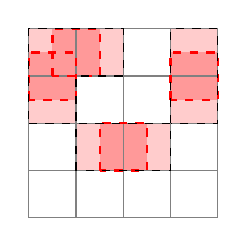
\begin{tikzpicture}[scale=0.3] 
    % Define parameters
    \def\xmin{0}
    \def\xmax{8}
    \def\ymin{0}
    \def\ymax{8}


    \fill[\stepOneColor] (2,2) rectangle (6, 4);
    \fill[\stepOneColor] (6,4) rectangle (8, 8);
    \fill[\stepOneColor] (0,4) rectangle (2, 8);
    \fill[\stepOneColor] (2,6) rectangle (4, 8);
    
    
    \fill[\fillerColor] (3,2) rectangle (5, 4);
    \fill[\fillerColor] (6,5) rectangle (8,7);
    \fill[\fillerColor] (0,5) rectangle (2,7);
    \fill[\fillerColor] (1,6) rectangle (3,8);
    

    \draw[step=2.0,gray,thin] (\xmin,\ymin) grid (\xmax,\ymax);
    
    \draw[dashed,thick, red](3,2) rectangle (5, 4);
    \draw[dashed,thick, red](6,5) rectangle (8, 7);
    \draw[dashed,thick, red](0,5) rectangle (2, 7);
    \draw[dashed,thick, red](1,6) rectangle (3, 8);
    
    \draw[dashed, black] (0,4) -- (2,4) -- (2,6) -- (4,6) -- (4,8)  -- (0,8) -- (0,4);
    \draw[dashed, black] (2,2) rectangle (6,4);
    \draw[dashed, black] (6,4) rectangle (8,8);
\end{tikzpicture}
    \end{subfigure}
    \begin{subfigure}[b]{0.48\textwidth}
        \centering
        \caption{four neighbouring squares}
\label{Figure::filler_square_four}
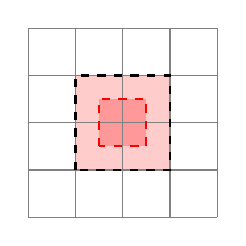
\begin{tikzpicture}[scale=0.3]
    % Define parameters
    \def\xmin{0}
    \def\xmax{8}
    \def\ymin{0}
    \def\ymax{8}

    \fill[\stepOneColor] (2,2) rectangle (6, 6);
    
    \fill[\fillerColor] (3,3) rectangle (5, 5);
    \draw[step=2.0,gray,thin] (\xmin,\ymin) grid (\xmax,\ymax);

    \draw[dashed,thick, red](3,3) rectangle (5, 5);
    
    \draw[dashed, thick, black](2,2) rectangle (6, 6);
\end{tikzpicture}
    \end{subfigure}

\end{figure}
    To get to the next stage, we keep the squares for the current stage and subdivide the grid further. Then we repeat the process of checking if any remaining uncovered squares (and their closures) fall under $U$ completely, and check if any filling is needed.
    Using this method, it is guaranteed that each point in $U$ will eventually be covered by these open squares. A visual trace for this algorithm on an open set is shown in Figure \ref{Figure::inner_decision}. Note that in this example, the search radius covers $U$ entirely from step 0.
    

\begin{figure}[H]
    \centering
    \caption{Visualization of the algorithm outputting an open exhaustion using a decision procedure}
    \label{Figure::inner_decision}

    \begin{subfigure}[b]{0.48\textwidth}
        \centering
        \caption{step 0}
\label{Figure::inner_decision_step0}
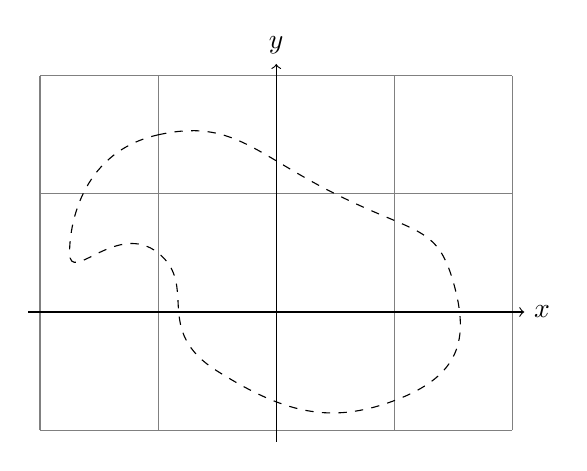
\begin{tikzpicture}[scale=0.75]

    % Define parameters
    \def\xmin{-4}
    \def\xmax{4}
    \def\ymin{-2}
    \def\ymax{4}

    \draw[step=2.0,gray,thin] (\xmin,\ymin) grid (\xmax,\ymax);

    % Axes
    \draw[->] (\xmin-0.2, 0) -- (\xmax+0.2, 0) node[right] {$x$};
    \draw[->] (0, \ymin-0.2) -- (0, \ymax+0.2) node[above] {$y$};
    
    \draw[dashed] plot [smooth cycle, tension=1] coordinates {(-3.5,1) (-2,3) (1,2) (3,0.5) (2,-1.5) (-1,-1)  (-2,1) };
\end{tikzpicture}

    \end{subfigure}
    \hfill
    \begin{subfigure}[b]{0.48\textwidth}
        \centering
        \caption{step 1}
\label{Figure::inner_decision_step1}
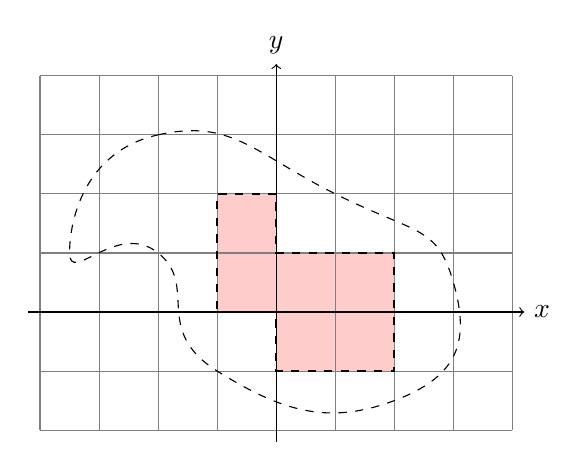
\begin{tikzpicture}[scale=0.75]
    % Define parameters
    \def\xmin{-4}
    \def\xmax{4}
    \def\ymin{-2}
    \def\ymax{4}

    % level 1
    \fill[\stepOneColor] (-1, 0) rectangle (0, 2);
    
    \fill[\stepOneColor]  (0, -1) rectangle (2, 1);
    
    \draw[step=1.0,gray,thin] (\xmin,\ymin) grid (\xmax,\ymax);

    % Axes
    \draw[->] (\xmin-0.2, 0) -- (\xmax+0.2, 0) node[right] {$x$};
    \draw[->] (0, \ymin-0.2) -- (0, \ymax+0.2) node[above] {$y$};
    
    \draw[dashed] plot [smooth cycle, tension=1] coordinates {(-3.5,1) (-2,3) (1,2) (3,0.5) (2,-1.5) (-1,-1)  (-2,1) };
    \draw[dashed, thick, black](-1,0) -- (0, 0) -- (0,-1) -- (2,-1) -- (2,1) -- (0,1) -- (0,2) -- (-1, 2) -- (-1,0);

\end{tikzpicture}

    \end{subfigure}

    \vspace{0.5cm} % Adjust spacing between rows if needed

    \begin{subfigure}[b]{0.48\textwidth}
        \centering
        \caption{step 2}
\label{Figure::inner_decision_step2}
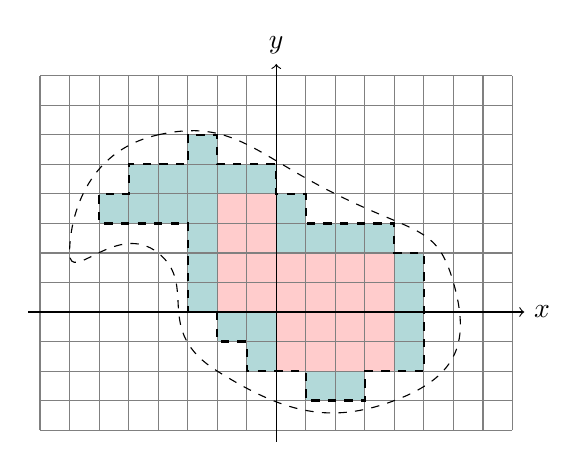
\begin{tikzpicture}[scale=0.75]

    % Define parameters
    \def\xmin{-4}
    \def\xmax{4}
    \def\ymin{-2}
    \def\ymax{4}

    % level 1
    \fill[\stepOneColor] (-1, 0) rectangle (0, 2);
    
    \fill[\stepOneColor] (0, -1) rectangle (2, 1);
    % level 2

    \fill[\stepTwoColor] (-1,-0.5) rectangle (-0.5,0);
    \fill[\stepTwoColor] (-0.5,-1) rectangle (0,0);
    \fill[\stepTwoColor] (0.5,-1.5) rectangle (1.5,-1);
    \fill[\stepTwoColor] (2,-1) rectangle (2.5,1);
    \fill[\stepTwoColor] (0,1) rectangle (2,1.5);
    \fill[\stepTwoColor] (0,1.5) rectangle (0.5,2);
    \fill[\stepTwoColor] (-1.5,0) rectangle (-1,3);
    \fill[\stepTwoColor] (-1,2) rectangle (0,2.5);
    \fill[\stepTwoColor] (-2.5,1.5) rectangle (-1.5,2.5);
    \fill[\stepTwoColor] (-3,1.5) rectangle (-2.5,2);

    \draw[step=.5,gray,thin] (\xmin,\ymin) grid (\xmax,\ymax);

    % Axes
    \draw[->] (\xmin-0.2, 0) -- (\xmax+0.2, 0) node[right] {$x$};
    \draw[->] (0, \ymin-0.2) -- (0, \ymax+0.2) node[above] {$y$};
    
    \draw[dashed] plot [smooth cycle, tension=1] coordinates {(-3.5,1) (-2,3) (1,2) (3,0.5) (2,-1.5) (-1,-1)  (-2,1) };
    \draw[dashed, thick, black](-1,0) -- (-1,-0.5) -- (-0.5, -0.5) -- (-0.5, -1) -- (0.5, -1) -- (0.5, -1.5) -- (1.5,-1.5) -- (1.5,-1) -- (1.5, -1) -- (2.5, -1) -- (2.5, 1) -- (2, 1) -- (2, 1.5) -- (0.5, 1.5) -- (0.5, 1.5) -- (0.5,2)--(0, 2) -- (0, 2.5) -- (-1, 2.5) -- (-1, 3) -- (-1.5, 3) -- (-1.5, 2.5) -- (-2.5, 2.5) -- (-2.5, 2) -- (-3, 2) -- (-3,1.5) -- (-1.5, 1.5) -- (-1.5,0) -- (-1,0);

\end{tikzpicture}

    \end{subfigure}
    \hfill
    \begin{subfigure}[b]{0.48\textwidth}
        \centering
        \caption{step 3}
\label{Figure::inner_decision_step3}
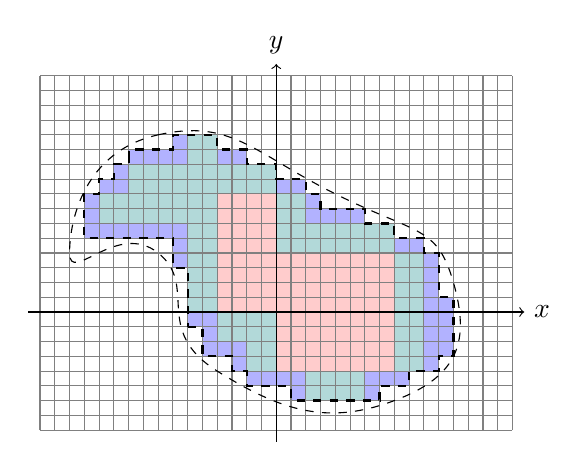
\begin{tikzpicture}[scale=0.75]

    % Define parameters
    \def\xmin{-4}
    \def\xmax{4}
    \def\ymin{-2}
    \def\ymax{4}

    % level 1
    \fill[\stepOneColor] (-1, 0) rectangle (0, 2);
    
    \fill[\stepOneColor] (0, -1) rectangle (2, 1);
    % level 2

    \fill[\stepTwoColor] (-1,-0.5) rectangle (-0.5,0);
    \fill[\stepTwoColor] (-0.5,-1) rectangle (0,0);
    \fill[\stepTwoColor] (0.5,-1.5) rectangle (1.5,-1);
    \fill[\stepTwoColor] (2,-1) rectangle (2.5,1);
    \fill[\stepTwoColor] (0,1) rectangle (2,1.5);
    \fill[\stepTwoColor] (0,1.5) rectangle (0.5,2);
    \fill[\stepTwoColor] (-1.5,0) rectangle (-1,3);
    \fill[\stepTwoColor] (-1,2) rectangle (0,2.5);
    \fill[\stepTwoColor] (-2.5,1.5) rectangle (-1.5,2.5);
    \fill[\stepTwoColor] (-3,1.5) rectangle (-2.5,2);
    % level 3
    \fill[\stepThreeColor] (-0.5,-1.25) rectangle (0.5,-1);
    \fill[\stepThreeColor] (0.25,-1.5) rectangle (0.5,-1.25);
    \fill[\stepThreeColor] (1.5,-1.5) rectangle (1.75,-1);
    \fill[\stepThreeColor] (1.75,-1.25) rectangle (2.25,-1);
    \fill[\stepThreeColor] (2.5,-1) rectangle (2.75,1);
    \fill[\stepThreeColor] (2.75,-0.75) rectangle (3,0.25);
    \fill[\stepThreeColor] (2,1) rectangle (2.5, 1.25);
    \fill[\stepThreeColor] (0.5,1.5) rectangle (1.5,1.75);
    \fill[\stepThreeColor] (0.5,1.75) rectangle (0.75, 2);
    \fill[\stepThreeColor] (0,2) rectangle (0.5, 2.25);
    \fill[\stepThreeColor] (-1,2.5) rectangle (-0.5, 2.75);
    \fill[\stepThreeColor] (-1.75,2.5) rectangle (-1.5, 3);
    \fill[\stepThreeColor] (-2.5, 2.5) rectangle (-1.75,2.75);
    \fill[\stepThreeColor] (-2.75,2) rectangle (-2.5, 2.5);
    \fill[\stepThreeColor] (-3,2) rectangle (-2.75, 2.25);
    \fill[\stepThreeColor] (-3.25,1.25) rectangle (-3,2);
    \fill[\stepThreeColor] (-3,1.25) rectangle (-1.5,1.5);
    \fill[\stepThreeColor] (-1.75,0.75) rectangle (-1.5, 1.25);
    \fill[\stepThreeColor] (-1.5, -0.25) rectangle (-1,0);
    \fill[\stepThreeColor] (-1.25, -0.75) rectangle (-1,-0.25);
    \fill[\stepThreeColor] (-1, -0.75) -- (-0.75,-0.75) -- (-0.75, -1) -- (-0.5, -1) -- (-0.5, -0.5) -- (-1, -0.5);

    \draw[step=.25,gray,thin] (\xmin,\ymin) grid (\xmax,\ymax);

    % Axes
    \draw[->] (\xmin-0.2, 0) -- (\xmax+0.2, 0) node[right] {$x$};
    \draw[->] (0, \ymin-0.2) -- (0, \ymax+0.2) node[above] {$y$};
    
    \draw[dashed] plot [smooth cycle, tension=1] coordinates {(-3.5,1) (-2,3) (1,2) (3,0.5) (2,-1.5) (-1,-1)  (-2,1) };

    \draw[dashed, thick, black](-1.5, -0.25) -- (-1.25, -0.25) -- (-1.25, -0.75) -- (-0.75, -0.75) -- (-0.75, -1) -- (-0.5, -1) -- (-0.5, -1.25) -- (0.25, -1.25) -- (0.25, -1.5) -- (1.75, -1.5) -- (1.75, -1.25) -- (2.25, -1.25) -- (2.25, -1) -- (2.75, -1) -- (2.75, -0.75) --(3, -0.75) -- (3, 0.25) -- (2.75, 0.25) -- (2.75, 1) -- (2.5, 1) -- (2.5, 1.25) -- (2, 1.25) -- (2, 1.5) -- (1.5, 1.5) -- (1.5, 1.75) -- (0.75, 1.75) -- (0.75, 2) -- (0.5, 2) --(0.5, 2.25) -- (0, 2.25) -- (0, 2.25)-- (0, 2.5) -- (-0.5, 2.5) -- (-0.5, 2.75) -- (-1, 2.75) -- (-1, 3) -- (-1.75, 3) -- (-1.75, 3) -- (-1.75, 2.75) -- (-2.5, 2.75) -- (-2.5, 2.5) -- (-2.5, 2.75) -- (-2.5, 2.5) -- (-2.75, 2.5) -- (-2.75, 2.25) -- (-3, 2.25) -- (-3, 2) -- (-3.25, 2) -- (-3.25, 1.25) -- (-1.75, 1.25) -- (-1.75, 0.75) -- (-1.5, 0.75) -- (-1.5, -0.25);
\end{tikzpicture}


    \end{subfigure}

\end{figure}
    Note that here the filler squares are not shown, and only the area that is covered at each stage is shown. Step 0 is when the algorithm starts. The output for stage 0 (resp.\null{} 1 and 2) is shown in step 1 (resp.\null{} 2 and 3). Different colors show in which stage the points are covered using the open exhaustion.

\end{proof}